\documentclass{article}

\usepackage{amsmath}
\usepackage{amsthm}
\usepackage{amssymb}
\usepackage{amsfonts}
\usepackage{graphics}
\usepackage{tikz}
\usepackage{hyperref}
\usepackage{graphicx}
\usepackage{enumerate}
\usepackage{color}
\usepackage{mathtools}
\usepackage{stmaryrd}

\usepackage{pgf, latexsym, float, soul, array, booktabs, dsfont, gensymb, wasysym, multicol}

\usepackage[margin=1in]{geometry}

% set font encoding for PDFLaTeX, XeLaTeX, or LuaTeX
\usepackage{ifxetex,ifluatex}
\if\ifxetex T\else\ifluatex T\else F\fi\fi T%
  \usepackage{fontspec}
\else
  \usepackage[T1]{fontenc}
  \usepackage[utf8]{inputenc}
  \usepackage{lmodern}
\fi

\usepackage{hyperref}


\newcommand{\N}{\mathbb{N}}
\newcommand{\Z}{\mathbb{Z}}
\newcommand{\Zz}{\mathcal{Z}}
\newcommand{\R}{\mathbb{R}}
\newcommand{\Q}{\mathbb{Q}}
\newcommand{\C}{\mathbb{C}}
\newcommand{\PP}{\mathbb{P}}
\newcommand{\X}{\mathcal{X}}
\newcommand{\B}{\mathcal{B}}
\newcommand{\A}{\mathcal{A}}
\newcommand{\M}{\mathcal{M}}
\newcommand{\NN}{\mathcal{N}}
\newcommand{\F}{\mathcal{F}}
\newcommand{\E}{\mathcal{E}}
\newcommand{\ELL}{\mathcal{ELL}}
\renewcommand{\O}{\mathcal{O}}
\renewcommand{\H}{\mathcal{H}}
\newcommand{\D}{\mathbb{D}}
\newcommand{\dabba}{\partial}
\newcommand{\e}{\epsilon}
\newcommand{\eu}{\text{e}}
\newcommand{\bs}{\blacksquare}
\newcommand{\di}{\diamond}
\newcommand{\lb}{\left\lbrace}
\newcommand{\rb}{\right\rbrace}
\newcommand{\on}[1]{\operatorname{#1}}
\newcommand{\lcm}{\on{lcm}}
\newcommand{\multichoose}[2]{\left[#1\atop #2\right]}
\newcommand{\Aut}{\operatorname{Aut}}
\newcommand{\Inn}{\operatorname{Inn}}
\renewcommand{\Im}{\operatorname{Im}}
\newcommand{\Cl}{\operatorname{Cl}}
\newcommand{\Int}{\operatorname{Int}}
\newcommand{\id}{\operatorname{id}}





\theoremstyle{definition}
\newtheorem{theorem}{Theorem}[section]
\newtheorem{proposition}[theorem]{Proposition}
\newtheorem{corollary}[theorem]{Corollary}
\newtheorem{lemma}[theorem]{Lemma}

\newtheorem*{theorem*}{Theorem}



\newtheorem*{problem}{Problem}
\newtheorem*{fact}{Fact}
\newtheorem*{claim}{Claim}
\newtheorem*{exercise}{Exercise}

\theoremstyle{definition}
\newtheorem*{definition}{Definition}
\newtheorem*{remark}{Remark}
\newtheorem*{question}{Question}






\title{Calculus 1 Notes and Thoughts \\ Spring 2022}
\author{Peter E. Francis}

\begin{document}
\maketitle

\tableofcontents

\newpage

\section{Limits}

Limits are very important in Calculus, since we need very small quantities to effectively study change. Yeah, that's pretty vague, but hopefully it'll clear up in a few pages.

We study limits for many reasons. One of them is to study functions at points where they are not defined, but are ``close'' to being defined. For example, the function $f$ given by $f(x)=\frac{x(x+1)}{x}$ is not defined at $0$, but looks like the line $x+1$ everywhere else.

\subsection{Intuitive Limits}

The important idea of a \textbf{limit} is to examine what the output of a function does as the input moves close to a specific value. Since the functions that we will be studying are from $\R$ to $\R$, and there are two ways that you can approach a number on the real line (from the left and right) we will talk about left- and right-sided limits.

Before getting into the actual definition, we'll start intuitively. If a function is     ``continuous''\footnote{I put this word in quotes because I haven't defined it yet, but you should have an intuitive idea of what this means: being able to draw it without lifting your pencil. Just wait for a few pages.} and is defined at $a$, then as $x$ moves closer to $a$, $f(x)$ moves closer to $f(a)$, so the limit of $f$ as $x$ approaches $a$ is $f(a)$.


Let's get a little more general: suppose a function $f$ is defined on open intervals on either side of $a$.

\begin{center}
\def\arraystretch{1.1}
\begin{tabular}{| p{2.25in} | p{2.25in} |} \hline
If $f$ is defined on an interval to the \textbf{left} of $a$ and the values of $f(x)$ approach $L$ as $x$ approaches $a$ from the \textbf{left}, we say that the ``\textbf{left}-sided limit of $f$ as $x$ approaches $a$ is $L$'' and we write $$\lim_{x\to a^-}f(x)=L.$$ & If $f$ is defined on an interval to the \textbf{right} of $a$ and the values of $f(x)$ approach $L$ as $x$ approaches $a$ from the \textbf{right}, we say that the ``\textbf{right}-sided limit of $f$ as $x$ approaches $a$ is $L$'' and we write
$$\lim_{x\to a^+}f(x)=L.$$
\\\hline
\multicolumn{2}{| p{4.5in} |}{If the right and left sided limits match, then we say that the ``limit of $f$ as $x$ approaches $a$ is $L$'' and write $$\lim_{x\to a}f(x)=L.$$} \\\hline
\end{tabular}
\end{center}

\noindent Note: $f$ need not be defined at $a$ to evaluate the limit of $f$ as $x$ approaches $a$.

\vspace{1em}

One can compute $f(x)$ for values of $x$ that get closer and closer to either side of $a$. If the values approach $L$, then you have good reason to believe that $L$ is the (right- and/or left-sided) limit.

\begin{center}
\begin{tabular}{| c | c |}
\hline
   $x$        & $f(x)$        \\\hline\hline
   $a-0.1$    & $f(a-0.1)$    \\\hline
   $a-0.01$   & $f(a-0.01)$   \\\hline
   $a-0.001$  & $f(a-0.001)$  \\\hline
   $a-0.0001$ & $f(a-0.0001)$ \\\hline\hline
   $a+0.0001$ & $f(a+0.0001)$ \\\hline
   $a+0.001$  & $f(a+0.001)$  \\\hline
   $a+0.01$   & $f(a+0.01)$   \\\hline
   $a+0.1$    & $f(a+0.1)$    \\\hline
\end{tabular}
\end{center}

Such calculations, however, cannot prove that a function limits to a specific value.

\subsection{Infinite Limits}

We can extend the idea of limits outside of the real numbers to include positive and negative infinity in place of both $a$ and $L$.
\begin{itemize}
\item If $f(x)$ grows (in the $\pm$ direction) without bound as $x$ approaches $a$ from the left, then we write $$\lim_{x\to a^-}f(x)=\pm\infty.$$
Similarly for $x$ approaching $a$ from the right.
\item We denote the value (if such a value exists) that $f(x)$ approaches as $x$ approaches $\pm\infty$ as $$\lim_{x\to\pm\infty} f(x).$$
\end{itemize}



\subsection{The $\epsilon-\delta$ Definition}

You may be dissatisfied with the intuitive approach to limits, so we'll make the definition more rigorous. The main idea that needs to be captured by a formal definition is \textit{arbitrary precision}. That is, we need a way to say formally that ``$f(x)$ approaches $L$ as $x$ approaches $a$.''

By controlling the input $x$, we must be able to make the distance $|f(x)-L|$ between the output $f(x)$ and $L$ to be as small as we want (``arbitrarily small''). In other words, if $\epsilon>0$ is any small positive number, we must be able to ensure (by controlling $x$) that $|f(x)-L| < \epsilon$. To control $x$, we can make the distance $|x-a|$ between $x$ and $a$ smaller than some positive number $\delta > 0$ (that may depend on $\epsilon$).

Now we're ready for the real ``$\epsilon-\delta$'' definition of a limit: we say that \textbf{$L$ is the limit of $f$ as $x$ approaches $a$} if
$$\text{for all } \epsilon > 0, \text{ there exists some } \delta > 0, \text{ such that } |x - a| < \delta \implies |f(x) - L| <\epsilon.$$

Read that last line a few times, because statements with multiple quantifiers can be tricky! It may be helpful to think about the definition of a limit as a game/conversation between two people, Alex and Blake. Alex is trying to claim that the limit of $f$ as $x\to a$ is L, and Blake is doing their best job to contest it. Here is how their conversation might go:
\begin{itemize}
\item[A:] I think the limit of $f(x)=3x+1$ as $x$ approaches $2$ is 7.
\item[B:] Well if you think so, then can you ensure that $|f(x)-7|<\frac{1}{10}$?
\item[A:] Yes! If we take $x$ such that $|x-2|<1/30$, then
$$|f(x)-7|=|3x + 1 - 7| = |3x-6| = 3|x-2| < 3(1/30) = 1/10.$$
\end{itemize}
In this example, $\epsilon = 1/10$ and $\delta = 1/30$. However, if we want to really prove that the limit is 7, we let $\epsilon>0$ be arbitrary, and take $\delta = \epsilon/3$. Then for any $x$ such that $|x-2|<\delta$,
$$|f(x)-7|=|3x + 1 - 7| = |3x-6| = 3|x-2| < 3(\epsilon/3) = \epsilon.$$

For simple examples, it is pretty easy to work backwards and figure out what $\delta$ should be, but for more complicated functions $f$, it can be more difficult. Here is a \href{https://www.desmos.com/calculator/cuoca85inx}{Desmos example} that shows dynamically how $\delta$ can depend on $\epsilon$.


\newpage
\subsection{Limit Laws}

So far we have used the $\epsilon-\delta$ definition to prove that a limit of a function is a certain value, we estimated limits using computation, and we might be able to eye-ball a limit of a ``continuous'' function, but we still need a more sophisticated way to figure out what the limit of a function is at a certain point. There are several \textit{limit laws} that make computing limits easier. We also have two basic facts that should be obvious: for any $a,b\in \R$,

$$\lim_{x\to a} b = b \quad\text{ and }\quad \lim_{x\to a}x=a.$$

Together with the following laws, you'll be able to evaluate the limits of many functions. Suppose $\displaystyle\lim _{x \to a} f(x)=L$ and $\displaystyle\lim _{x \to a} g(x)=M$, and let $c$ be a constant. Then the following hold.


\begin{center}
\def\arraystretch{2.5}
\begin{tabular}{| p{1.75in} | p{3.75in} |}
\hline
\textbf{Sum law} & $\displaystyle\lim _{x \rightarrow a}(f(x)+g(x))=\lim _{x \rightarrow a} f(x)+\lim _{x \rightarrow a} g(x)=L+M$ \\ \hline
\textbf{Difference law} & $\displaystyle\lim _{x \rightarrow a}(f(x)-g(x))=\lim _{x \rightarrow a} f(x)-\lim _{x \rightarrow a} g(x)=L-M$ \\ \hline
\textbf{Constant multiple law} & $\displaystyle\lim _{x \rightarrow a} c f(x)=c \cdot \lim _{x \rightarrow a} f(x)=c L$ \\ \hline
\textbf{Product law} & $\displaystyle\lim _{x \rightarrow a}(f(x) \cdot g(x))=\lim _{x \rightarrow a} f(x) \cdot \lim _{x \rightarrow a} g(x)=L \cdot M$ \\ \hline
\textbf{Quotient law} & $\displaystyle\lim _{x \rightarrow a} \frac{f(x)}{g(x)}=\frac{\displaystyle\lim _{x \rightarrow a} f(x)}{\displaystyle\lim _{x \rightarrow a} g(x)}=\frac{L}{M}$ for $M \neq 0$ \\ \hline
\textbf{Power law} & $\displaystyle\lim _{x \rightarrow a}(f(x))^{n}=\left(\lim _{x \rightarrow a} f(x)\right)^{n}=L^{n}$ for every positive integer $n$. \\ \hline
\textbf{Root law} & $\displaystyle\lim _{x \rightarrow a} \sqrt[n]{f(x)}=\sqrt[n]{\lim _{x \rightarrow a} f(x)}=\sqrt[n]{L}$ for all $L$ if $n$ is odd and for $L \geq 0$ if $n$ is even and $f(x) \geq 0 .$
\\\hline
\end{tabular}

\end{center}

\subsection{Limit ``Tricks'' and Key Examples}

There are some other tricks that will help you evaluate limits. Try these things if you're not sure what else to do; they might be helpful if you end up in a situation where you are trying to divide 0/0.
\begin{itemize}
\item Simplify. Perhaps the function is rational, and has common factor in its numerator and denominator. By ``canceling'' the term, the resulting function is not the same: the original function has a hole at the point where the factored term is 0. For example, $f(x)=\frac{x(x-1)}{(x-1)}$ has a hole at $x=1$, but everywhere else is the line $y=x$.
\item Multiply by the conjugate of the denominator or the numerator of a rational function (the conjugate of a binomial $a+b$ is $a-b$).
\item $\displaystyle\lim_{x\to 0}\frac{\sin(x)}{x} = 1$.
\item $\displaystyle\lim_{x\to 0}\frac{\cos(x) - 1}{x} = 0$.
\item $\displaystyle\lim_{x\to\infty}\left(1+\frac{1}{x}\right)^x = e$.
\end{itemize}





\newpage

\section{Continuity}

\subsection{Definitions}

A function $f:\R\to\R$ is \textbf{continuous at $a$} if three conditions are satisfied:
\begin{enumerate}[(a)]
\item $f$ is defined at $a$ (i.e. $f(a)$ makes sense)
\item $\displaystyle\lim_{x\to a^+} f(x)= f(a)$
\item $\displaystyle\lim_{x\to a^-} f(x)= f(a)$
\end{enumerate}
If (a), (b), or (c) are not true, then $f$ is \textbf{discontinuous at $a$}. There are three types of discontinuities: if $f$ is discontinuous at $a$, then
\begin{enumerate}[1.]
\item $f$ has a \textbf{removable discontinuity} at $a$ if $\displaystyle\lim _{x \to a} f(x)$ exists and is a real number.
\item $f$ has a \textbf{jump discontinuity} at $a$ if $\displaystyle\lim _{x \to a^{-}} f(x)$ and $\displaystyle\lim _{x \to a^{+}} f(x)$ both exist and are real numbers, but are different.
\item $f$ has an \textbf{infinite discontinuity} at $a$ if $\displaystyle\lim _{x \to a^{-}} f(x)=\pm \infty$ or $\displaystyle\lim _{x \to a^{+}} f(x)=\pm \infty$.
\end{enumerate}

\subsection{Using Continuity}

The following functions are continuous at every point in their domains:
\begin{itemize}
\item polynomials
\item rational functions
\item trig and inverse trig functions
\item exponential functions
\item logarithms
\end{itemize}

Therefore, if you want to evaluate a limit of any of these functions $f$ at a point $a$ in its domain, the limit is equal to $f(a)$ since $f$ is continuous.

\vspace{1em}

\noindent Here's another limit law, now that you know about continuous functions:

\begin{theorem*}[Composite Function Theorem]
If $f(x)$ is continuous at $L$ and $\displaystyle\lim _{x \to a} g(x)=L$, then
$$\lim _{x \to a} f(g(x))=f\left(\lim _{x \to a} g(x)\right)=f(L).$$
\end{theorem*}

\noindent To finish off the section, a very useful theorem:

\begin{theorem*}[The Intermediate Value Theorem]
Let $f$ be continuous over a closed, bounded interval $[a, b]$. If $z$ is any real number between $f(a)$ and $f(b)$, then there is a number $c$ in $[a, b]$ satisfying $f(c)=z$.
\end{theorem*}



\newpage

\section{The Derivative}

\subsection{The Limit Definition}

\begin{multicols}{2}

Recall that a \textbf{secant line} is a line between two points on the graph of a function. If $f$ is a function and $(a,f(a))$ and $(b,f(b))$ are \textit{different} points on the function, then the secant line that they determine has equation
$$y=f(a) + \frac{f(b)-f(a)}{b-a}(x-a).$$
We can assume $b>a$ and write $b=a+h$ for some $h>0$. Then the equation for the secant line through $(a,f(a))$ and $(b,f(b))=(a+h,f(a+h))$ is
$$y=f(a) + \frac{f(a+h)-f(a)}{h}(x-a).$$


Now we're going to use \textit{limits} to move one point $(b,f(b))$ closer to the other $(a,f(a))$, and see what happens to the secant line. Since the secant line passes through the point $(a,f(a))$, we only have to track what happens to the slope. As $b$ moves to $a$, the value of $h$ goes to $0$, so the slope of the secant line approaches
$$\lim_{h\to 0}\frac{f(a+h)-f(a)}{h}.$$
We'll denote this quantity $f'(a)$, and call this the \textbf{derivative of $f$ at $a$} (if this limit exists). The line through the point $(a,f(a))$ with slope $f'(a)$ is called the \textbf{tangent line of $f$ at $a$} and has equation
$$y=f(a)+f'(a)(x-a).$$

\columnbreak

\resizebox{2.8in}{!}{

\tikzset{every picture/.style={line width=0.75pt}}

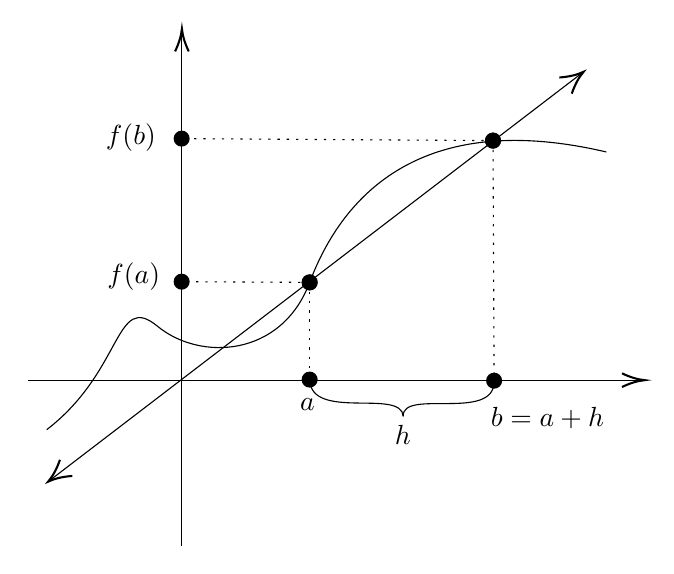
\begin{tikzpicture}[x=0.75pt,y=0.75pt,yscale=-1,xscale=1]
%uncomment if require: \path (0,441); %set diagram left start at 0, and has height of 441

%Straight Lines [id:da16102953695521127] 
\draw    (163,221.33) -- (458,221.33) ;
\draw [shift={(460,221.33)}, rotate = 180] [color={rgb, 255:red, 0; green, 0; blue, 0 }  ][line width=0.75]    (10.93,-3.29) .. controls (6.95,-1.4) and (3.31,-0.3) .. (0,0) .. controls (3.31,0.3) and (6.95,1.4) .. (10.93,3.29)   ;
%Straight Lines [id:da9043079513680581] 
\draw    (237.04,301) -- (237.04,54) ;
\draw [shift={(237.04,52)}, rotate = 90] [color={rgb, 255:red, 0; green, 0; blue, 0 }  ][line width=0.75]    (10.93,-3.29) .. controls (6.95,-1.4) and (3.31,-0.3) .. (0,0) .. controls (3.31,0.3) and (6.95,1.4) .. (10.93,3.29)   ;
%Curve Lines [id:da7565789477512073] 
\draw    (171.9,245.19) .. controls (209.02,216.63) and (204.74,178.41) .. (225.27,195.34) .. controls (245.8,212.28) and (284.99,210.33) .. (298.59,174.22) .. controls (312.18,138.1) and (347.09,89.21) .. (441.52,111.39) ;
%Straight Lines [id:da9796385406474812] 
\draw    (428.99,73.97) -- (174.17,269.02) ;
\draw [shift={(172.58,270.23)}, rotate = 322.57] [color={rgb, 255:red, 0; green, 0; blue, 0 }  ][line width=0.75]    (10.93,-4.9) .. controls (6.95,-2.3) and (3.31,-0.67) .. (0,0) .. controls (3.31,0.67) and (6.95,2.3) .. (10.93,4.9)   ;
\draw [shift={(430.57,72.75)}, rotate = 142.57] [color={rgb, 255:red, 0; green, 0; blue, 0 }  ][line width=0.75]    (10.93,-4.9) .. controls (6.95,-2.3) and (3.31,-0.67) .. (0,0) .. controls (3.31,0.67) and (6.95,2.3) .. (10.93,4.9)   ;
%Straight Lines [id:da4030910320179846] 
\draw  [dash pattern={on 0.84pt off 2.51pt}]  (298.59,174.22) -- (298.59,221.05) ;
\draw [shift={(298.59,221.05)}, rotate = 90] [color={rgb, 255:red, 0; green, 0; blue, 0 }  ][fill={rgb, 255:red, 0; green, 0; blue, 0 }  ][line width=0.75]      (0, 0) circle [x radius= 3.35, y radius= 3.35]   ;
\draw [shift={(298.59,174.22)}, rotate = 90] [color={rgb, 255:red, 0; green, 0; blue, 0 }  ][fill={rgb, 255:red, 0; green, 0; blue, 0 }  ][line width=0.75]      (0, 0) circle [x radius= 3.35, y radius= 3.35]   ;
%Straight Lines [id:da14103701021608472] 
\draw  [dash pattern={on 0.84pt off 2.51pt}]  (386.93,105.91) -- (387.46,221.58) ;
\draw [shift={(387.46,221.58)}, rotate = 89.74] [color={rgb, 255:red, 0; green, 0; blue, 0 }  ][fill={rgb, 255:red, 0; green, 0; blue, 0 }  ][line width=0.75]      (0, 0) circle [x radius= 3.35, y radius= 3.35]   ;
\draw [shift={(386.93,105.91)}, rotate = 89.74] [color={rgb, 255:red, 0; green, 0; blue, 0 }  ][fill={rgb, 255:red, 0; green, 0; blue, 0 }  ][line width=0.75]      (0, 0) circle [x radius= 3.35, y radius= 3.35]   ;
%Curve Lines [id:da47143485860977985] 
\draw    (298.59,221.05) .. controls (299.18,241.14) and (342.98,225.16) .. (343.66,238.75) ;
%Curve Lines [id:da42610723931770456] 
\draw    (387.46,221.58) .. controls (388.06,241.67) and (342.98,225.16) .. (343.66,238.75) ;
%Straight Lines [id:da3483526368480112] 
\draw  [dash pattern={on 0.84pt off 2.51pt}]  (298.59,174.22) -- (236.91,173.88) ;
\draw [shift={(236.91,173.88)}, rotate = 180.32] [color={rgb, 255:red, 0; green, 0; blue, 0 }  ][fill={rgb, 255:red, 0; green, 0; blue, 0 }  ][line width=0.75]      (0, 0) circle [x radius= 3.35, y radius= 3.35]   ;
\draw [shift={(298.59,174.22)}, rotate = 180.32] [color={rgb, 255:red, 0; green, 0; blue, 0 }  ][fill={rgb, 255:red, 0; green, 0; blue, 0 }  ][line width=0.75]      (0, 0) circle [x radius= 3.35, y radius= 3.35]   ;
%Straight Lines [id:da4035786093366658] 
\draw  [dash pattern={on 0.84pt off 2.51pt}]  (386.93,105.91) -- (236.91,104.95) ;
\draw [shift={(236.91,104.95)}, rotate = 180.37] [color={rgb, 255:red, 0; green, 0; blue, 0 }  ][fill={rgb, 255:red, 0; green, 0; blue, 0 }  ][line width=0.75]      (0, 0) circle [x radius= 3.35, y radius= 3.35]   ;
\draw [shift={(386.93,105.91)}, rotate = 180.37] [color={rgb, 255:red, 0; green, 0; blue, 0 }  ][fill={rgb, 255:red, 0; green, 0; blue, 0 }  ][line width=0.75]      (0, 0) circle [x radius= 3.35, y radius= 3.35]   ;

% Text Node
\draw (292.79,228.73) node [anchor=north west][inner sep=0.75pt]    {$a$};
% Text Node
\draw (384.59,233.05) node [anchor=north west][inner sep=0.75pt]    {$b=a+h$};
% Text Node
\draw (338.35,242.02) node [anchor=north west][inner sep=0.75pt]    {$h$};
% Text Node
\draw (199.88,163.44) node [anchor=north west][inner sep=0.75pt]    {$f( a)$};
% Text Node
\draw (199.19,96.46) node [anchor=north west][inner sep=0.75pt]    {$f( b)$};


\end{tikzpicture}

}

\vspace{2em}

\resizebox{2.8in}{!}{

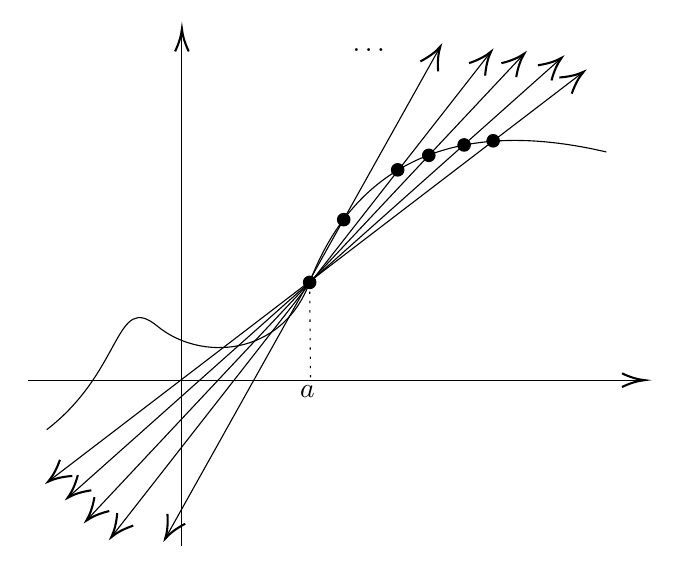
\begin{tikzpicture}[x=0.75pt,y=0.75pt,yscale=-1,xscale=1]
%uncomment if require: \path (0,441); %set diagram left start at 0, and has height of 441

%Straight Lines [id:da16102953695521127] 
\draw    (163,221.33) -- (458,221.33) ;
\draw [shift={(460,221.33)}, rotate = 180] [color={rgb, 255:red, 0; green, 0; blue, 0 }  ][line width=0.75]    (10.93,-3.29) .. controls (6.95,-1.4) and (3.31,-0.3) .. (0,0) .. controls (3.31,0.3) and (6.95,1.4) .. (10.93,3.29)   ;
%Straight Lines [id:da9043079513680581] 
\draw    (237.04,301) -- (237.04,54) ;
\draw [shift={(237.04,52)}, rotate = 90] [color={rgb, 255:red, 0; green, 0; blue, 0 }  ][line width=0.75]    (10.93,-3.29) .. controls (6.95,-1.4) and (3.31,-0.3) .. (0,0) .. controls (3.31,0.3) and (6.95,1.4) .. (10.93,3.29)   ;
%Curve Lines [id:da7565789477512073] 
\draw    (171.9,245.19) .. controls (209.02,216.63) and (204.74,178.41) .. (225.27,195.34) .. controls (245.8,212.28) and (284.99,210.33) .. (298.59,174.22) .. controls (312.18,138.1) and (347.09,89.21) .. (441.52,111.39) ;
%Straight Lines [id:da9796385406474812] 
\draw    (428.99,73.97) -- (174.17,269.02) ;
\draw [shift={(172.58,270.23)}, rotate = 322.57] [color={rgb, 255:red, 0; green, 0; blue, 0 }  ][line width=0.75]    (10.93,-4.9) .. controls (6.95,-2.3) and (3.31,-0.67) .. (0,0) .. controls (3.31,0.67) and (6.95,2.3) .. (10.93,4.9)   ;
\draw [shift={(430.57,72.75)}, rotate = 142.57] [color={rgb, 255:red, 0; green, 0; blue, 0 }  ][line width=0.75]    (10.93,-4.9) .. controls (6.95,-2.3) and (3.31,-0.67) .. (0,0) .. controls (3.31,0.67) and (6.95,2.3) .. (10.93,4.9)   ;
%Straight Lines [id:da1158565706067487] 
\draw    (384.77,64.58) -- (204.23,295.42) ;
\draw [shift={(203,297)}, rotate = 308.03] [color={rgb, 255:red, 0; green, 0; blue, 0 }  ][line width=0.75]    (10.93,-4.9) .. controls (6.95,-2.3) and (3.31,-0.67) .. (0,0) .. controls (3.31,0.67) and (6.95,2.3) .. (10.93,4.9)   ;
\draw [shift={(386,63)}, rotate = 128.03] [color={rgb, 255:red, 0; green, 0; blue, 0 }  ][line width=0.75]    (10.93,-4.9) .. controls (6.95,-2.3) and (3.31,-0.67) .. (0,0) .. controls (3.31,0.67) and (6.95,2.3) .. (10.93,4.9)   ;
%Straight Lines [id:da7715304094905251] 
\draw    (400.63,65.46) -- (192.37,287.54) ;
\draw [shift={(191,289)}, rotate = 313.16] [color={rgb, 255:red, 0; green, 0; blue, 0 }  ][line width=0.75]    (10.93,-4.9) .. controls (6.95,-2.3) and (3.31,-0.67) .. (0,0) .. controls (3.31,0.67) and (6.95,2.3) .. (10.93,4.9)   ;
\draw [shift={(402,64)}, rotate = 133.16] [color={rgb, 255:red, 0; green, 0; blue, 0 }  ][line width=0.75]    (10.93,-4.9) .. controls (6.95,-2.3) and (3.31,-0.67) .. (0,0) .. controls (3.31,0.67) and (6.95,2.3) .. (10.93,4.9)   ;
%Straight Lines [id:da44730990962603356] 
\draw    (418.51,67.33) -- (183.49,276.67) ;
\draw [shift={(182,278)}, rotate = 318.31] [color={rgb, 255:red, 0; green, 0; blue, 0 }  ][line width=0.75]    (10.93,-4.9) .. controls (6.95,-2.3) and (3.31,-0.67) .. (0,0) .. controls (3.31,0.67) and (6.95,2.3) .. (10.93,4.9)   ;
\draw [shift={(420,66)}, rotate = 138.31] [color={rgb, 255:red, 0; green, 0; blue, 0 }  ][line width=0.75]    (10.93,-4.9) .. controls (6.95,-2.3) and (3.31,-0.67) .. (0,0) .. controls (3.31,0.67) and (6.95,2.3) .. (10.93,4.9)   ;
%Shape: Circle [id:dp8153494409622872] 
\draw  [fill={rgb, 255:red, 0; green, 0; blue, 0 }  ,fill opacity=1 ] (384,106) .. controls (384,104.34) and (385.34,103) .. (387,103) .. controls (388.66,103) and (390,104.34) .. (390,106) .. controls (390,107.66) and (388.66,109) .. (387,109) .. controls (385.34,109) and (384,107.66) .. (384,106) -- cycle ;
%Shape: Circle [id:dp46038093787284295] 
\draw  [fill={rgb, 255:red, 0; green, 0; blue, 0 }  ,fill opacity=1 ] (370,108) .. controls (370,106.34) and (371.34,105) .. (373,105) .. controls (374.66,105) and (376,106.34) .. (376,108) .. controls (376,109.66) and (374.66,111) .. (373,111) .. controls (371.34,111) and (370,109.66) .. (370,108) -- cycle ;
%Shape: Circle [id:dp190859565625209] 
\draw  [fill={rgb, 255:red, 0; green, 0; blue, 0 }  ,fill opacity=1 ] (353,113) .. controls (353,111.34) and (354.34,110) .. (356,110) .. controls (357.66,110) and (359,111.34) .. (359,113) .. controls (359,114.66) and (357.66,116) .. (356,116) .. controls (354.34,116) and (353,114.66) .. (353,113) -- cycle ;
%Shape: Circle [id:dp3044800797092422] 
\draw  [fill={rgb, 255:red, 0; green, 0; blue, 0 }  ,fill opacity=1 ] (338,120) .. controls (338,118.34) and (339.34,117) .. (341,117) .. controls (342.66,117) and (344,118.34) .. (344,120) .. controls (344,121.66) and (342.66,123) .. (341,123) .. controls (339.34,123) and (338,121.66) .. (338,120) -- cycle ;
%Shape: Circle [id:dp7651386739199335] 
\draw  [fill={rgb, 255:red, 0; green, 0; blue, 0 }  ,fill opacity=1 ] (295.59,174.22) .. controls (295.59,172.56) and (296.93,171.22) .. (298.59,171.22) .. controls (300.24,171.22) and (301.59,172.56) .. (301.59,174.22) .. controls (301.59,175.87) and (300.24,177.22) .. (298.59,177.22) .. controls (296.93,177.22) and (295.59,175.87) .. (295.59,174.22) -- cycle ;
%Straight Lines [id:da21925282533113744] 
\draw  [dash pattern={on 0.84pt off 2.51pt}]  (298.59,174.22) -- (299,221) ;
%Straight Lines [id:da4492754198498514] 
\draw    (360.57,62.35) -- (229.98,295.92) ;
\draw [shift={(229,297.67)}, rotate = 299.21] [color={rgb, 255:red, 0; green, 0; blue, 0 }  ][line width=0.75]    (10.93,-4.9) .. controls (6.95,-2.3) and (3.31,-0.67) .. (0,0) .. controls (3.31,0.67) and (6.95,2.3) .. (10.93,4.9)   ;
\draw [shift={(361.54,60.61)}, rotate = 119.21] [color={rgb, 255:red, 0; green, 0; blue, 0 }  ][line width=0.75]    (10.93,-4.9) .. controls (6.95,-2.3) and (3.31,-0.67) .. (0,0) .. controls (3.31,0.67) and (6.95,2.3) .. (10.93,4.9)   ;
%Shape: Circle [id:dp18797969215530874] 
\draw  [fill={rgb, 255:red, 0; green, 0; blue, 0 }  ,fill opacity=1 ] (312,144) .. controls (312,142.34) and (313.34,141) .. (315,141) .. controls (316.66,141) and (318,142.34) .. (318,144) .. controls (318,145.66) and (316.66,147) .. (315,147) .. controls (313.34,147) and (312,145.66) .. (312,144) -- cycle ;

% Text Node
\draw (292.79,222.73) node [anchor=north west][inner sep=0.75pt]    {$a$};
% Text Node
\draw (318,60.4) node [anchor=north west][inner sep=0.75pt]    {$\dotsc $};


\end{tikzpicture}

}

\end{multicols}


You'll notice that the tangent line captures some \textit{local information} about $f$ at $a$. In other words, it is a good approximation of $f$ at $a$; that is, $f$ and its tangent line are ``similar'' at $a$. Intuitively, you should think about the tangent line at $a$ to be the line that ``hugs $f$ the best.''

Note that this definition of the derivative only makes sense if $f$ is defined on an open interval containing $a$. We can view the derivative as a function, and write $f'(x)$. The derivative of $f'(x)$ is called the \textbf{second derivative} and is denoted $f''(x)$. In general, the $n$th derivative $f^{(n)}(x)$ is defined to be the derivative of $f^{(n-1)}(x)$. Other notation is sometimes used: if $y=f(x)$, $\frac{dy}{dx}=\frac{d}{dx}[f(x)]$ is the derivative of $f$, and $\frac{d^ny}{dx^n}=\frac{d^n}{dx^n}[f(x)]$ is the $n$th derivative of $f$.


\newpage

\subsection{The Two Part ``Program'' for Finding Derivatives}

So now we have a goal: find derivatives of functions. The problem is that the limit definition is difficult to use (that pesky $h\to 0$ in the denominator). So instead, we will do the following two steps (let $a$ be a real number):
\begin{enumerate}
\item ``break functions up into simpler ones''

\begin{center}
\def\arraystretch{1.5}
\begin{tabular}{| l | l |}
\hline
\textbf{The Scalar Multiple Rule} & $(au)' = au'$. \\ \hline
\textbf{The Sum Rule} & $(u + v)' = u' + v'$ \\ \hline
\textbf{The Product Rule} & $(uv)' = u'v + uv'$ \\ \hline
\textbf{The Quotient Rule} & $\left(\frac{u}{v}\right)' = \frac{u'v - uv'}{v^2}$ \\ \hline
\end{tabular}
\end{center}

\item find derivatives of ``simple'' functions:

\begin{center}
\def\arraystretch{1.5}
\begin{tabular}{| l | l |}
\hline
\textbf{The Constant Rule}     & $\frac{d}{dx}[a] = 0$ \\ \hline
\textbf{The Power Rule}        & $\frac{d}{dx}[x^a] = ax^{a-1}$ \\ \hline
\textbf{Basic Trig Functions}  & $\frac{d}{dx}[\sin(x)] = \cos(x)$ and $\frac{d}{dx}[\cos(x)] = -\sin(x)$ \\ \hline
\textbf{Exponential Functions} & $\frac{d}{dx}[a^x] = \ln(a)a^x$ \\ \hline
\textbf{Logarithmic Functions} & $\frac{d}{dx}[\log_a(x)] = \frac{1}{x\ln(a)}$ \\
\hline
\end{tabular}
\end{center}

\end{enumerate}

Most of the time, you will be able to find the derivatives using a combination of these rules. For instance, the derivatives of the other 4 trig functions can be found using the quotient rule and the derivatives of $\sin$ and $\cos$:
$$\frac{d}{dx}[\tan(x)] = \sec^2(x)
\quad\quad\quad\quad\quad
\frac{d}{dx}[\sec(x)] = \sec(x)\tan(x)$$

$$\frac{d}{dx}[\cot(x)] = -\csc^2(x)
\quad\quad\quad\quad\quad
\frac{d}{dx}[\csc(x)] = -\csc(x)\cot(x)$$

% \begin{itemize}
% \item 
% \end{itemize}



\subsection{Comparing the Graphs of $f$, $f'$, and $f''$}

\begin{center}
\def\arraystretch{1.5}
\begin{tabular}{| c | c | c |}
\hline
$f$ & $f'$ & $f''$ \\ \hline\hline

increasing & positive & \\ \hline
constant & 0 & \\ \hline
decreasing & negative & \\ \hline \hline

concave up & increasing & positive \\ \hline
linear & constant & 0 \\ \hline
concave down & decreasing & negative \\ \hline \hline

% Inflection point & constant & 0 \\ \hline
% local extrema & 0 & \\ \hline
% \hline

\end{tabular}
\end{center}




































\end{document}
